\documentclass[english,reprint, aps, prl,superscriptaddress, showpacs,
showkeys, longbibliography, amsmath, amssymb, floatfix]{revtex4-1} 
\pdfoutput=1

\usepackage{fullpage}
\usepackage{cmap}
\usepackage[T1,T2A]{fontenc}
\usepackage[utf8]{inputenc}
\usepackage[french,main=english]{babel}
\usepackage{amsthm}
\usepackage{mathrsfs}
\usepackage{bbold}
\usepackage{wesa}
\usepackage{graphicx}
\usepackage{verbatim}
\usepackage[backref=false]{hyperref}
\usepackage{booktabs}
\usepackage{multirow}
\usepackage[braket,qm]{qcircuit}
\usepackage{color}
\usepackage[usenames,dvipsnames]{xcolor}
\usepackage{framed}
\usepackage{comment}
\usepackage{xparse}

\theoremstyle{plain}
\newtheorem{thm}{Theorem}
\newtheorem{lemma}{Lemma}[thm]
\newtheorem{cor}{Corollary}[thm]
\newtheorem{assumption}{Assumption}
\newtheorem{fact}{Fact}
\theoremstyle{definition}
\newtheorem{definition}{Definition}
\newtheorem{condition}[assumption]{Condition}

\DeclareUnicodeCharacter{0229}{\c{e}}

\newcommand{\Hilb}{\mathcal{H}}
\newcommand{\events}{\ensuremath{\mathcal{E}}}
\newcommand{\qevents}{\ensuremath{\mathcal{E}}}
\newcommand{\pmeas}{\ensuremath{\mu}}
% \newcommand{\imposs}{{\text{\wesa{impossible}}}}
% \newcommand{\likely}{{\text{\wesa{likely}}}}
% \newcommand{\unlikely}{{\text{\wesa{unlikely}}}}
% \newcommand{\necess}{{\text{\wesa{certain}}}}
% \newcommand{\unknown}{{\text{\wesa{unknown}}}}
% \newcommand{\midd}{{\text{\wesa{middle}}}}
\newcommand{\imposs}{\ensuremath{\left[0,0\right]}}
\newcommand{\likely}{\ensuremath{\left[\tfrac{1}{2},1\right]}}
\newcommand{\unlikely}{\ensuremath{\left[0,\tfrac{1}{2}\right]}}
\newcommand{\necess}{\ensuremath{\left[1,1\right]}}
\newcommand{\unknown}{\ensuremath{\left[0,1\right]}}
\newcommand{\midd}{\ensuremath{\left[\tfrac{1}{4},\tfrac{3}{4}\right]}}
\newcommand{\fket}[1]{{|#1\rangle}}
\newcommand{\fproj}[1]{|#1\rangle\langle #1|}
\newcommand{\proj}[1]{\op{#1}{#1}}
\newcommand{\ps}{\texttt{+}}
\newcommand{\ms}{\texttt{-}}
\newcommand{\set}[2]{\ensuremath{\left\{ {#1}\mathrel{}\middle|\mathrel{}{#2}\right\} }}
\newcommand{\Tr}{\ensuremath{\mathop{\mathrm{Tr}}\nolimits}}
\allowdisplaybreaks
\newcommand{\coreBorn}{\ensuremath{\overline{\Hilb}}}
\newcommand{\mul}[1][]{\ensuremath{\mu^{L{#1}}}}
\newcommand{\mur}[1][]{\ensuremath{\mu^{R{#1}}}}
\setcounter{secnumdepth}{3}
% https://tex.stackexchange.com/questions/345284/can-i-have-an-almost-non-breaking-space-in-latex
% Change non-breaking space to \nolinebreak[1] 
% Hence, it will not hyphenate too much surrounding words.
\newcommand{\rmd}{d}
\newcommand{\rmi}{i}
\lineskiplimit=1pt
\newcommand{\ultramodular}{\mathcal{M}}
\newcommand{\ultramodularL}[1][]{\ensuremath{\ultramodular^{L{#1}}}}
\newcommand{\ultramodularR}[1][]{\ensuremath{\ultramodular^{R{#1}}}}
\newcommand{\muB}{\ensuremath{\mu^{B}}}
\newcommand{\eventsC}{\ensuremath{\events_{C}}}

\newcommand{\says}[3]{\begin{framed}\begin{minipage}{0.9\linewidth}\color{#1}{#2 says: #3}\end{minipage}\end{framed}}
\newcommand{\amr}[1]{\says{green}{Amr}{#1}}
\newcommand{\yutsung}[1]{\says{purple}{Yu-Tsung}{#1}}
\newcommand{\gerardo}[1]{\says{OliveGreen}{Gerardo}{#1}}
\newcommand{\andy}[1]{\says{blue}{Andy}{#1}}
% \excludecomment{suggest}
\NewDocumentEnvironment{suggest}{m m O{}}{#1{TEXT \##2 would go here. #3}}{#1{TEXT \##2 end here.}}

\newcommand{\happen}{\text{H}}
\newcommand{\notHappen}{\text{N}}
\newcommand{\missing}{\text{M}}
%%%%%%%%%%%%%%%%%%%%%%%%%%%%%%%%%%%%%%%%%%%%%%%%%%%%%%%%%%%%%%%%%%%
\begin{document}

\title{Response to the Referee Report of ``Quantum Interval-Valued Probability:
Contextuality and the Born Rule''}

\author{Yu-Tsung Tai}

\affiliation{Department of Mathematics, Indiana University, Bloomington, Indiana
47405, USA}

\affiliation{Department of Computer Science, Indiana University, Bloomington,
Indiana 47405, USA}

\author{Andrew J. Hanson}

\affiliation{Department of Informatics, Indiana University, Bloomington, Indiana
47405, USA}

\author{Gerardo Ortiz}

\affiliation{Department of Physics, Indiana University, Bloomington, Indiana 47405,
USA}

\author{Amr Sabry}

\affiliation{Department of Computer Science, Indiana University, Bloomington,
Indiana 47405, USA}

\date{\today}

\maketitle
%%%%%%%%%%%%%%%%%%%%%%%%%%%%%%%%%%%%%%%%%%%%%%%%%%%%%%%%%%%%%%%%%%%

\section{Finite-precision Extension of the Kochen-Specker Theorem}

\begin{thm}[Finite-precision Extension of the Kochen-Specker Theorem]
\label{cor:Kochen-Specker-IVPM} Given a Hilbert space $\Hilb$ of
dimension~$d\ge3$, there is no $\delta$-deterministic QIVPM for
$\delta<\frac{1}{3}$.\end{thm}

The proof is by contradiction: Suppose there is a $\delta$-deterministic
QIVPM~$\bar{\mu}:\events\rightarrow\mathscr{I}$. Now use this assumed
QIVPM to construct the following $0$-deterministic QIVPM $\bar{\mu}^{\textrm{D}}:\events\rightarrow\left\{ \imposs,\necess\right\} $:
\begin{equation}
\bar{\mu}^{\textrm{D}}\left(P\right)=\begin{cases}
\imposs\,, & \textrm{ if }\bar{\mu}\left(P\right)\subseteq\left[0,\delta\right]\:;\\
\necess\,, & \textrm{ if }\bar{\mu}\left(P\right)\subseteq\left[1-\delta,1\right]\:.
\end{cases}
\end{equation}
However, since we know that $0$-deterministic QIVPMs do not exist,
the map $\bar{\mu}^{\textrm{D}}$ cannot exist and hence $\bar{\mu}$
does not exist. It remains to verify that $\bar{\mu}^{\textrm{D}}$
is indeed a QIVPM by checking that for orthogonal projectors $P_{0}$
and~$P_{1}$, 
\begin{equation}
\bar{\mu}^{\textrm{D}}\left(P_{0}+P_{1}\right)=\bar{\mu}^{\textrm{D}}\left(P_{0}\right)+\bar{\mu}^{\textrm{D}}\left(P_{1}\right)\,,\label{eq:QuantumInterval-valuedProbability-Equal}
\end{equation}
because Eq.~(\ref{eq:QuantumInterval-valuedProbability-Equal}) implies
the convexity condition.

When one of $\bar{\mu}^{\textrm{D}}\left(P_{0}\right)$ and $\bar{\mu}^{\textrm{D}}\left(P_{1}\right)$
is $\necess$, say $\bar{\mu}^{\textrm{D}}\left(P_{0}\right)=\necess$
and $\bar{\mu}^{\textrm{D}}\left(P_{1}\right)=\imposs$, we have $\bar{\mu}\left(P_{0}\right)\subseteq\left[1-\delta,1\right]$
and $\bar{\mu}\left(P_{1}\right)\subseteq\left[0,\delta\right]$ which
implies $\bar{\mu}\left(P_{0}+P_{1}\right)\subseteq\left[1-\delta,1+\delta\right]$.
Since $\bar{\mu}\left(P_{0}+P_{1}\right)$ is a subset of $\left[0,1\right]$,
$\bar{\mu}\left(P_{0}+P_{1}\right)$ must be a subset of $\left[1-\delta,1\right]$,
which implies $\bar{\mu}^{\textrm{D}}\left(P_{0}+P_{1}\right)=\necess$.

\begin{figure*}
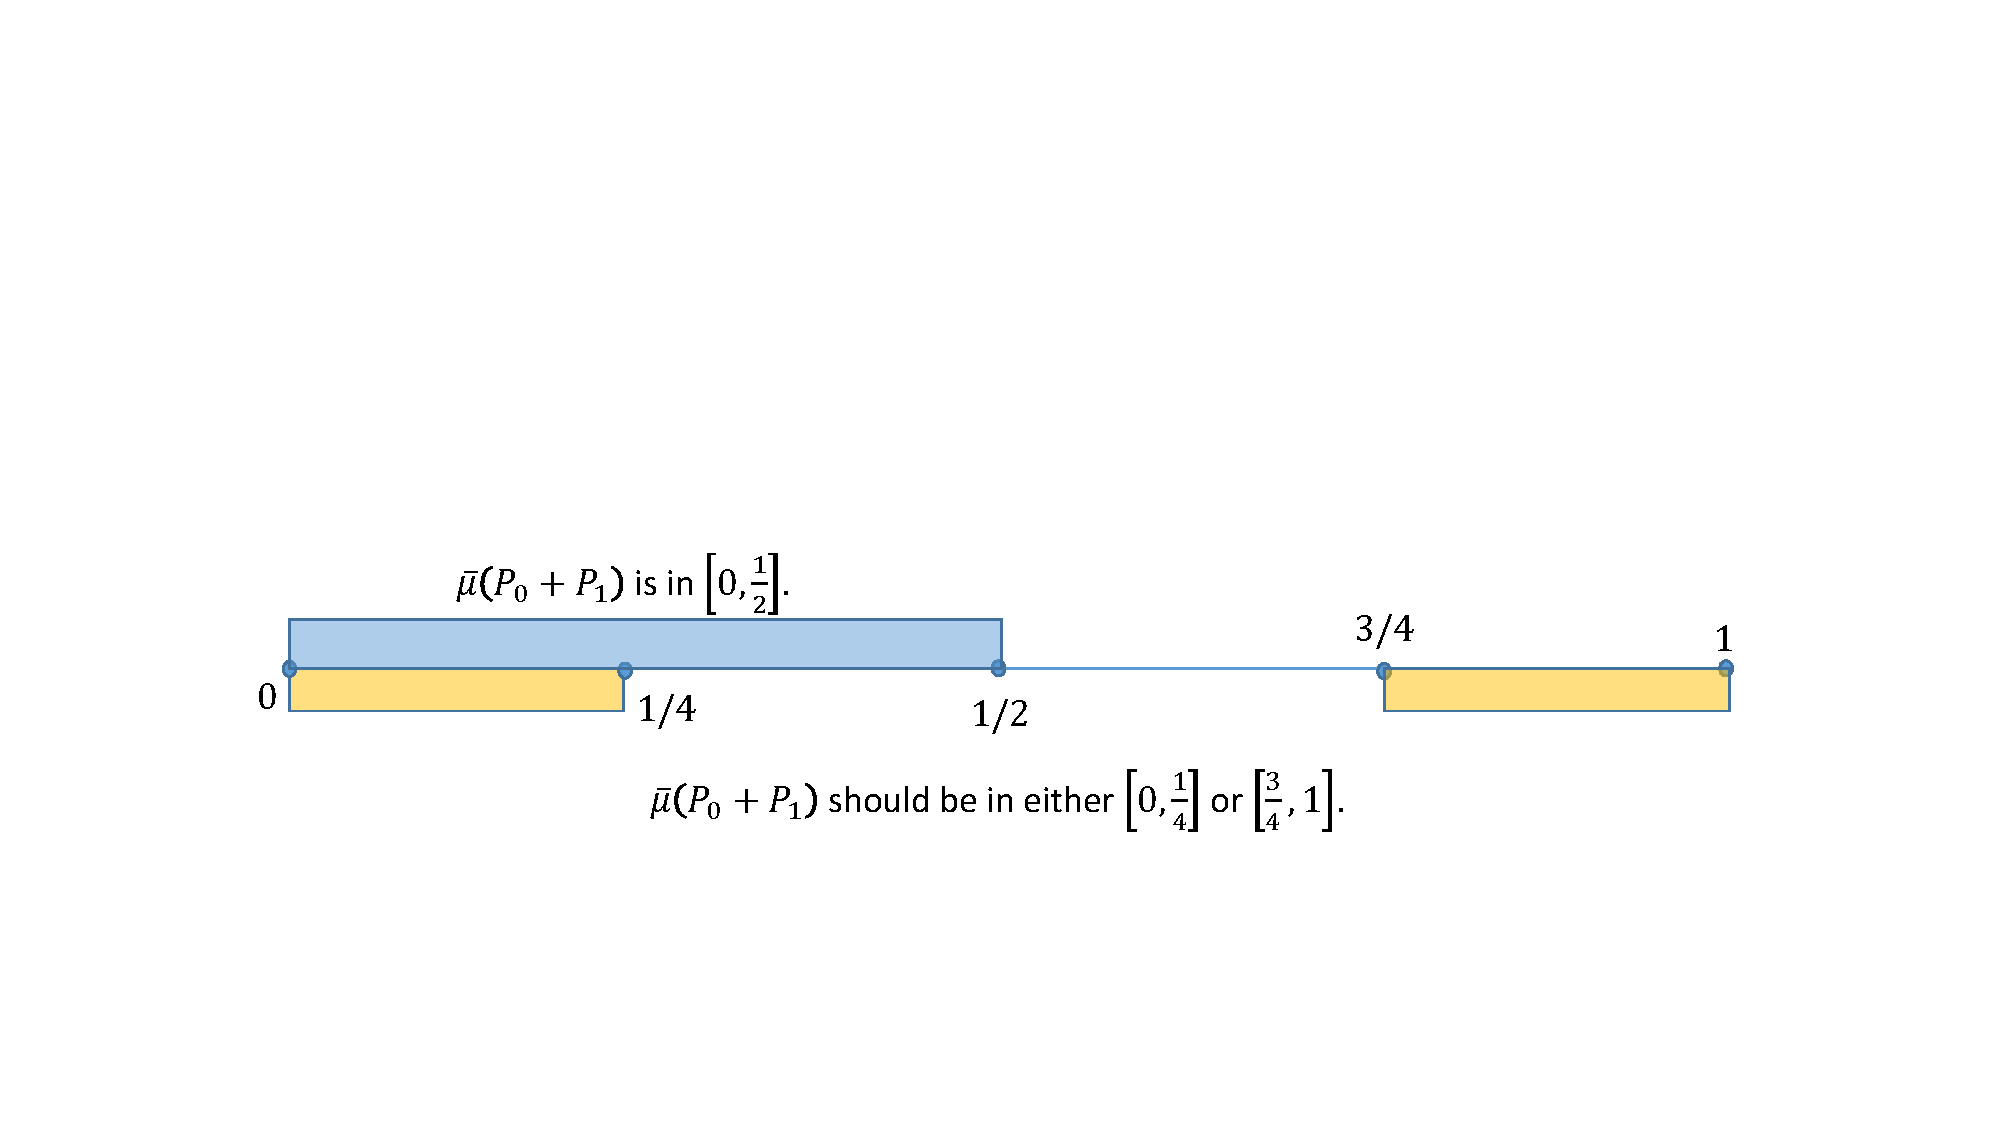
\includegraphics[bb=50bp 100bp 900bp 300bp,clip,scale=0.5]{prop_prop_letter_ajhs_referee_response_pptx}\caption{\label{fig:Show-subset}Since $\bar{\mu}\left(P_{0}+P_{1}\right)$
and $\left[1-\delta,1\right]$ are disjoint, $\bar{\mu}\left(P_{0}+P_{1}\right)$
is a subset of $\left[0,\delta\right]$.}
\end{figure*}
When $\bar{\mu}^{\textrm{D}}\left(P_{0}\right)=\bar{\mu}^{\textrm{D}}\left(P_{1}\right)=\imposs$,
we have both $\bar{\mu}\left(P_{0}\right)$ and $\bar{\mu}\left(P_{1}\right)\subseteq\left[0,\delta\right]$
which implies $\bar{\mu}\left(P_{0}+P_{1}\right)\subseteq\left[0,2\delta\right]$.
Since $\bar{\mu}\left(P_{0}+P_{1}\right)$ is a subset of either $\left[0,\delta\right]$
or $\left[1-\delta,1\right]$ and the latter is excluded as illustrated
in Fig.~\ref{fig:Show-subset} , then $\bar{\mu}\left(P_{0}+P_{1}\right)$
must be a subset of $\left[0,\delta\right]$, which implies $\bar{\mu}^{\textrm{D}}\left(P_{0}+P_{1}\right)=\imposs$.

\section{Mermin-Peres ``Magic Square''}

In our response, we provide an example to show that if enough experimental
records are missing, there exists a probability measure consistent
with the experimental records. In this section, we want to provide
a similar example on the same nine observables $\mathbf{O}_{ij}$
with $i$ and $j$ ranging over $\{0,1,2\}$ from the Mermin-Peres
``magic square'' used to prove the Kochen-Specker theorem~\cite{Mermin1990Simple,peres1995quantum,Griffiths2003}:


{{\renewcommand{\arraystretch}{2}% 
\begin{center} 
\begin{tabular}{r|@{\quad}c@{\quad}|@{\quad}c@{\quad}|@{\quad}c@{\quad}|} 
$\mathbf{O}_{ij}$~ & $j=0$ & $j=1$ & $j=2$ \\ 
\hline  
$i=0~$ & $\mathbb{1}\otimes\sigma_{z}$  & $\sigma_{z}\otimes\mathbb{1}$  & $\sigma_{z}\otimes\sigma_{z}$ \tabularnewline 
\hline  
$i=1~$ & $\sigma_{x}\otimes\mathbb{1}$  & $\mathbb{1}\otimes\sigma_{x}$  & $\sigma_{x}\otimes\sigma_{x}$ \tabularnewline 
\hline  
$i=2~$ & $\sigma_{x}\otimes\sigma_{z}$  & $\sigma_{z}\otimes\sigma_{x}$  & $\sigma_{y}\otimes\sigma_{y}$ \tabularnewline 
\hline  
\end{tabular}\,.
\par\end{center} 
}

\noindent The observables are constructed using the Pauli matrices
$\left\{ \mathbb{1},\sigma_{x},\sigma_{y},\sigma_{z}\right\} $ whose
eigenvalues are all either~$1$ or $-1$ \cite{Redhead1987-REDINA,544199,Griffiths2003,Jaeger2007,Mermin2007}.
They are arranged such that in each row and column, \emph{except the
column $j=2$}, every observable is the product of the other two,
so does the expectation value of every observable is the product of
the other two. In the $j=2$ column, we have instead that $\left(\sigma_{z}\otimes\sigma_{z}\right)\left(\sigma_{x}\otimes\sigma_{x}\right)=-\sigma_{y}\otimes\sigma_{y}$
and $\expval{\mathbf{O}_{12}}\expval{\mathbf{O}_{22}}=-\expval{\mathbf{O}_{22}}$.

Assume we measure each observable twice. By the Kochen-Specker theorem,
the following measurement results is impossible because $\expval{\mathbf{O}_{12}}\expval{\mathbf{O}_{22}}=1\ne-1=-\expval{\mathbf{O}_{22}}$.
\begin{center}
\begin{tabular}{ccc}
\toprule 
\addlinespace
$\mathbf{O}_{ij}$  & Trial~0 & Trial~1\tabularnewline
\midrule
\midrule 
\addlinespace
$\mathbf{O}_{00}$ , $\mathbf{O}_{01}$, $\mathbf{O}_{10}$ , $\mathbf{O}_{11}$  & $-1$ & $-1$\tabularnewline
\midrule 
\addlinespace
$\mathbf{O}_{02}$ , $\mathbf{O}_{12}$ , $\mathbf{O}_{20}$ , $\mathbf{O}_{21}$
, $\mathbf{O}_{22}$  & $1$ & $1$\tabularnewline
\bottomrule
\end{tabular}
\par\end{center}

However, if half of the records are missing, i.e., $\delta=\frac{1}{2}$,
we might get the following measurement results, where $\missing$
stands for missing data.
\begin{center}
\begin{tabular}{cccc}
\toprule 
\addlinespace
$\mathbf{O}_{ij}$  & Trial~0 & Trial~1 & $\begin{aligned} & \textrm{Missing Record}\\
 & \textrm{Might Be}
\end{aligned}
$\tabularnewline
\midrule
\midrule 
\addlinespace
$\mathbf{O}_{00}$, $\mathbf{O}_{11}$ & $-1$ & $\missing$ & $1$\tabularnewline
\midrule 
\addlinespace
$\mathbf{O}_{01}$ , $\mathbf{O}_{10}$  & $\missing$ & $-1$ & $1$\tabularnewline
\midrule 
\addlinespace
$\mathbf{O}_{02}$ , $\mathbf{O}_{20}$ , $\mathbf{O}_{22}$  & $1$ & $\missing$ & $-1$\tabularnewline
\midrule 
\addlinespace
$\mathbf{O}_{12}$ , $\mathbf{O}_{21}$  & $\missing$ & $1$ & $-1$\tabularnewline
\bottomrule
\end{tabular}
\par\end{center}

Since the experimental results are missing, it might come form the
third column. In this kind of situation, the expectation values of
each observables is always $0$, and the product relations among these
the expectation values must be consistent with the the product relations
among observables.

We missed half of the experimental results when considering the Mermin-Peres
``magic square'' example, which is more than $\frac{1}{3}$ when
considering a three-dimensional Hilbert space. The reason is that
while there exists a $\frac{1}{3}$-deterministic QIVPMs in a three-dimensional
Hilbert space, we only know a $\frac{1}{2}$-deterministic QIVPMs,
but not any $\delta$-deterministic QIVPM for $\frac{1}{3}<\delta\le\frac{1}{2}$
in a four-dimensional Hilbert space.

%%%%%%%%%%%%%%%%%%%%%%%%%%%%%%%%%%%%%%%%%%%%%%%%%%%%%%%%%%%%%%%%%%%%%%%%%%%%%
\bibliography{prop}
\end{document}

